\documentclass[11pt,a4paper]{article}
\usepackage[utf8]{inputenc}
\usepackage[francais]{babel}
\usepackage[T1]{fontenc}
\usepackage{amsmath}
\usepackage{amsfonts}
\usepackage{amssymb}
\usepackage{graphicx}
\usepackage{wrapfig}
\usepackage[left=2cm,right=2cm,top=2cm,bottom=2cm]{geometry}
\author{Théophile \textsc{Bastian}, Noémie \textsc{Cartier}, Nathanaël \textsc{Courant}}

\usepackage{my_listings} % On aura besoin de mettre du code source, sûrement.
% Contient \lstbash{}, \lstocaml{}, \lstc{}, ... pour mettre du code inliné facilement

\usepackage{my_hyperref} % Hyperref (pour les URLs, hyperliens, ... cliquables et colorés non-dégueulassement)

\newcommand{\htodo}[1]{\begin{huge}\colorbox{yellow}{\textcolor{red}{\textbf{TODO~:} #1}}\end{huge}}
\newcommand{\todo}[1]{\colorbox{yellow}{\textcolor{red}{\textbf{TODO~:} #1}}}
\newcommand{\relire}{\colorbox{orange}{\textcolor{blue}{\textbf{RELIRE}~}}}
\newcommand{\relu}[1]{\colorbox{green}{\textcolor{red}{\textbf{RELU~:} #1}}}
%TODO pour le rendu, supprimer ces commandes et recompiler pour s'assurer de ne pas avoir laissé de TODO

\title{Rapport de projet -- Système digital}
\date{24 janvier 2016} % Date de rendu
\begin{document}
\maketitle

\relire
\relu{No}
\begin{abstract}
Notre objectif dans ce projet a été principalement d'avoir un code \emph{correct} et \emph{rapide à l'exécution}~; nous pensons avoir atteint ces deux objectifs. Dans ce but, nous avons commencé par implémenter non pas un simulateur, mais un \emph{compilateur} de netlists~; puis avons produit un code assembleur pour l'horloge extrêmement optimisé, tout en conservant un nombre constant de cycles processeur par incrément de seconde. Notre processeur en lui-même s'inspire fortement d'une architecture ARM, sans toutefois rechercher l'exhaustivité des opérations, ce qui nous a permis d'obtenir un processeur fonctionnel et composé de peu de portes, donc efficace. Pour finir, nous avons implémenté une GUI affichant un écran composé de blocs 7 segments, contrôlés directement par la sortie du processeur, optimisée jusqu'à ce que le programme limitant la vitesse d'exécution soit le processeur lui-même.

En définitive, les programmes obtenus, une fois combinés correctement, répondent bien au cahier des charges imposé et permettent d'atteindre une vitesse d'exécution en mode \textit{fast} de l'ordre de \textbf{3.5 jours simulées par seconde réelle}.
\end{abstract}

\setcounter{tocdepth}{2} % Limite la TOC à sections/subsections
\tableofcontents
\pagebreak


%%%%%%%%%%%%%%%%%%%%%%%%%%%%%%%%%%%%%%%%%%%%%%%%%%%%%
\section{Utilisation globale}
%%%%%%%%%%%%%%%%%%%%%%%%%%%%%%%%%%%%%%%%%%%%%%%%%%%%%

\todo{abstract ?}
\relire

\subsection{Utilisation}

La compilation de toutes les composantes du projet s'effectue simplement par un \lstbash{make} à la racine du projet. Les dépendances suivantes sont toutefois nécessaires~:

\begin{itemize}
\item OCaml~: \lstbash{ocamlbuild}, \lstbash{ocamlopt}, \lstbash{ocamllex}, \lstbash{menhir}
\item C~: \lstbash{gcc}
\item C++~: \lstbash{g++}
\item Python~: \lstbash{python3}
\item Qt version $\geq 4$, \lstbash{qmake}
\item Un environnement bash
\end{itemize}

Le lancement de l'horloge peut se faire dans trois modes~:
\begin{itemize}
\item temps réel~: \lstbash{make run} ou \lstbash{./run_realtime.sh}, horloge en temps réel synchronisée sur le temps système à l'initialisation~;
\item rapide~: \lstbash{make run-fast} ou \lstbash{./run_fast.sh}, horloge en accéléré initialisée sur le temps système~;
\item très rapide~: \lstbash{make run-very-fast} ou \lstbash{./run_very_fast.sh}, horloge en accélérée non-initialisée sur le temps système, ce qui permet de lui fournir comme entrée \texttt{/dev/null}, doublant presque les performances.
\end{itemize}

\subsection{Organisation du projet}

Les éléments du projet sont répartis dans des dossiers comme il suit~:
\begin{itemize}
\item \texttt{assember}~: l'assembleur pour notre processeur (§\ref{sec:cas})
\item \texttt{clock}~: les codes assembleur de nos programmes d'horloge (§\ref{sec:clock})
\item \texttt{display\_gui}~: l'interface d'affichage (§\ref{sec:gui})
\item \texttt{processor}~: le code produisant la netlist de notre processeur (§\ref{sec:proc})
\item \texttt{simulator}~: le compilateur de netlists (§\ref{sec:compilo})
\end{itemize}

%%%%%%%%%%%%%%%%%%%%%%%%%%%%%%%%%%%%%%%%%%%%%%%%%%%%%
\section{Compilateur de circuits} \label{sec:compilo}
%%%%%%%%%%%%%%%%%%%%%%%%%%%%%%%%%%%%%%%%%%%%%%%%%%%%%

\htodo{Nathanaël}

\todo{Abstract}

\subsection{Utilisation}
\todo{Commandes, \ldots}

\subsection{Fonctionnement}

\subsection{Entrées/sorties} \label{ssec:compilo_io}

\subsection{Optimisations}
\todo{Parce que ça a beau être dégueu, ça a la classe d'en parler :D}

%%%%%%%%%%%%%%%%%%%%%%%%%%%%%%%%%%%%%%%%%%%%%%%%%%%%%
\section{Processeur} \label{sec:proc}
%%%%%%%%%%%%%%%%%%%%%%%%%%%%%%%%%%%%%%%%%%%%%%%%%%%%%

\relire

Nous avons fait le choix d'écrire notre processeur en Python~: le code, une fois exécuté, produit un fichier de netlist qui peut être compilé avec le compilateur de circuits (§\ref{sec:compilo}). Le code a été conçu modulairement, avec un fichier Python par sous-unité du processeur (ALU, \ldots). Le fichier \lstbash{main.py} se charge donc exclusivement de faire le lien entre ces unités, \og branchant \fg{} des fils d'une unité à l'autre~; tandis que \lstbash{netlist.py} définit les fonctions à appeler pour construire la netlist en mémoire, affichable à la fin.

\htodo{Tout le monde}

%%%%%%%%%%%%%%%%%%%%%%%
\subsection{Architecture du processeur}

\subsubsection{Mémoires et registres} \label{sssec:memory}
\todo{RAM, ROM, registres (dont PC)}
\subsubsection{Opcodes} \label{sssec:opcodes}
\subsubsection{Opérations assembleur supportées}

%%%%%%%%%%%%%%%%%%%%%%%
\subsection{Détail des unités}

\subsubsection{ALU}
\todo{No}

Grâce à un choix adapté des opcodes pour les bonnes opérations, on limite ici le nombre de multiplexeurs utilisés.

L'ALU commence par déterminer les $op_1$ et $op_2$ adaptés à l'opération considérée~:
\begin{itemize}

\item si le dernier bit de l'instruction est un $1$ (vrai dans le cas de \lstc{SUB} et \lstc{BIC}), l'$op_2$ utilisé sera la négation de celui fournit par l'op2selector (en prenant en compte la retenue dans le cas de la soustraction, on retrouve bien l'opposé de l'$op_2$ donné à la base)~;

\item si le deuxième bit de l'instruction est un $1$, et uniquement dans le cas des opérations arithmétiques (donc seulement das le cas de l'opération \lstc{RSB}), l'$op_1$ utilisé sera la négation de celui fourni par l'op1selector.

\end{itemize}

L'ALU calcule ensuite séparément les résultats de toutes les opérations booléennes ainsi qu'un unique résultat arithmétique, qui sera une addition ou une soustraction (dans un sens ou dans l'autre) en fonction des $op_1$ et $op_2$ sélectionnés plus tôt. Nous justifions cette séparation par le fait qu'une structure d'additionneur est suffisamment importante pour la limiter à une unique occurrence, alors que les différente opérations booléennes, en plus d'être difficile à combiner (à l'exception de \lstc{AND} et \lstc{BIC}, qui l'ont été), sont nettement moins coûteuses en terme de nombre de portes logiques.

Enfin, l'ALU sélectionne la bonne sortie parmi toutes celles calculées. En particulier, un troisième bit à $0$ indique une opération arithmétique, tandis qu'un $1$ indique une opération booléenne.

\subsubsection{Flags unit}
\todo{Théo}

\subsubsection{Memory unit}
\todo{(qui, déjà ?)}

\subsubsection{$op_1$ unit}
\todo{Théo}

\subsubsection{$op_2$ unit}
\todo{Théo}

\subsubsection{Opcode unit}
\todo{Théo}

\subsubsection{Registers unit}
\todo{Nath}

\subsubsection{Result selector}
\todo{No (?)}

Il ne s'agit ici que d'un multiplexeur~: si l'instruction a son premier et son quatrième bit égaux à $1$, on sélectionne le résultat d'un accès mémoire~; sinon, on sélectionne le résultat donné par l'ALU.

%%%%%%%%%%%%%%%%%%%%%%%%%%%%%%%%%%%%%%%%%%%%%%%%%%%%%
\section{Assembleur} \label{sec:cas}
%%%%%%%%%%%%%%%%%%%%%%%%%%%%%%%%%%%%%%%%%%%%%%%%%%%%%

\htodo{Un peu tout le monde}

L'assembleur est très probablement la partie la plus simple de notre projet~: les opcodes (§\ref{sssec:opcodes}) utilisés sont très simples à construire, ainsi notre assembleur (programmé en OCaml) est constitué d'un lexer/parser, d'un traducteur d'AST en opcodes, d'un \og linker \fg{} gérant les sauts (\lstasm{JMP}) et d'un module écrivant la ROM (§\ref{sssec:memory}) finale.

\subsection{Gestion des sauts}
\todo{Nathanaël}

\vspace{1em}\htodo{D'autres subsections ?}


%%%%%%%%%%%%%%%%%%%%%%%%%%%%%%%%%%%%%%%%%%%%%%%%%%%%%
\section{Programme de l'horloge} \label{sec:clock}
%%%%%%%%%%%%%%%%%%%%%%%%%%%%%%%%%%%%%%%%%%%%%%%%%%%%%

\htodo{Nathanaël, qui va devoir être \emph{très} pédagogue}




%%%%%%%%%%%%%%%%%%%%%%%%%%%%%%%%%%%%%%%%%%%%%%%%%%%%%
\section{Interface de sortie} \label{sec:gui}
%%%%%%%%%%%%%%%%%%%%%%%%%%%%%%%%%%%%%%%%%%%%%%%%%%%%%

\relire

L'interface, programmée en C++ avec Qt, est composée de 14 afficheurs 7 segments, pilotés par l'entrée standard (détaillé ci-dessous §\ref{ssec:gui_use}). Elle supporte sans ralentissement les quelques $\sim 12\text{Mo}$ d'entrée par seconde en mode \emph{fast}.

\subsection{Utilisation} \label{ssec:gui_use}

La compilation s'effectue par un simple \lstbash{make} dans le dossier de l'interface (\texttt{display\_gui}), ou un \lstbash{make} dans le dossier du projet~; le binaire produit est \texttt{display\_gui/display\_gui}.

\begin{wrapfigure}{r}{0.35\textwidth}
\begin{center}
\vspace{-1em}
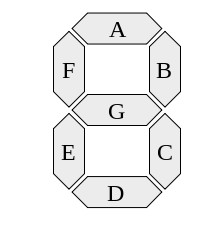
\includegraphics[width=0.2\textwidth]{imgs/7seg-labels.png}
\end{center}
\vspace{-2em}
\caption{Ordre des segments. Crédit~: H2g2bob @ Wikipedia}
\end{wrapfigure}

Le programme ne prend aucun argument. Il attend sur son entrée standard des caractères formatés comme la sortie du processeur (§\ref{ssec:compilo_io}), c'est-à-dire 16 caractères à la suite. Les caractères contrôlent chacun un afficheur, dans l'ordre \verb!--HHMMSSYYYYMMDD! respectivement heure à deux chiffres, minutes, secondes, année à 4 chiffres, mois, jour.

Les bits du caractère contrôlent les segments d'un afficheur, à savoir en commençant par les poids forts \verb!-gfedcba!

\subsection{Fonctionnement et optimisations}

La lecture de l'entrée standard est gérée dans un thread séparé du thread principal, se chargeant de l'affichage~; la communication entre threads est aisée puisque l'un est en écriture seule sur la mémoire partagée quand l'autre est en lecture seule.

Le thread d'affichage est volontairement limité à 30 FPS~: 30 fois par seconde, il demande au thread de lecture des valeurs pour chacun de ses segments et met à jour son interface. Ceci fut une première amélioration notable des performances, par rapport à un modèle où les segments sont rafraîchis aussi vite que possible.

Le thread de lecture, quant à lui, a été bien plus optimisé. Les modèles suivants ont été considérés, successivement~:
\begin{itemize}
\item Lorsque des valeurs sont demandées, on lit 16 caractères sur \lstc{stdin}~; lorsque le rafraîchissement est terminé, on \lstc{fflush} l'entrée standard afin d'ignorer ce qui est arrivé pendant ce temps. Cette option n'a jamais fonctionné, d'autant qu'elle ferait perdre tout repère de \og début de bloc de 16 caractères \fg{}.

\item On lit en continu des blocs de 16 caractères et, à chaque demande de rafraîchissement, on renvoie les 16 derniers acquis. Cette option marchait bien, mais était trop lente.

\item La \og boucle infinie \fg{} de lecture étant gérée avec Qt, le modèle signal/slot impose de faire en réalité une fonction de lecture se terminant par l'empilement d'un événement \og appeler la fonction de lecture \fg{}. Cette procédure est très coûteuse (beaucoup plus que \lstc{getchar}~!). Ainsi nous ignorons systématiquement 6 blocs sur 7~: la fonction de lecture lit $7 \times 16$ caractères et ne conserve que les 16 derniers. La fréquence de notre processeur nous permet (et nous oblige) à procéder de la sorte pour avoir une vitesse d'affichage raisonnable.
\end{itemize}

Avec ce fonctionnement, nous arrivons à une horloge capable de supporter l'entrée massive qui lui est fournie chaque seconde, sans ralentir le système global.

\end{document}